\chapter{基于并行的知识图谱与文本模型联合学习框架}
\label{cha:jointlearning}


\begin{figure}[]
\centering
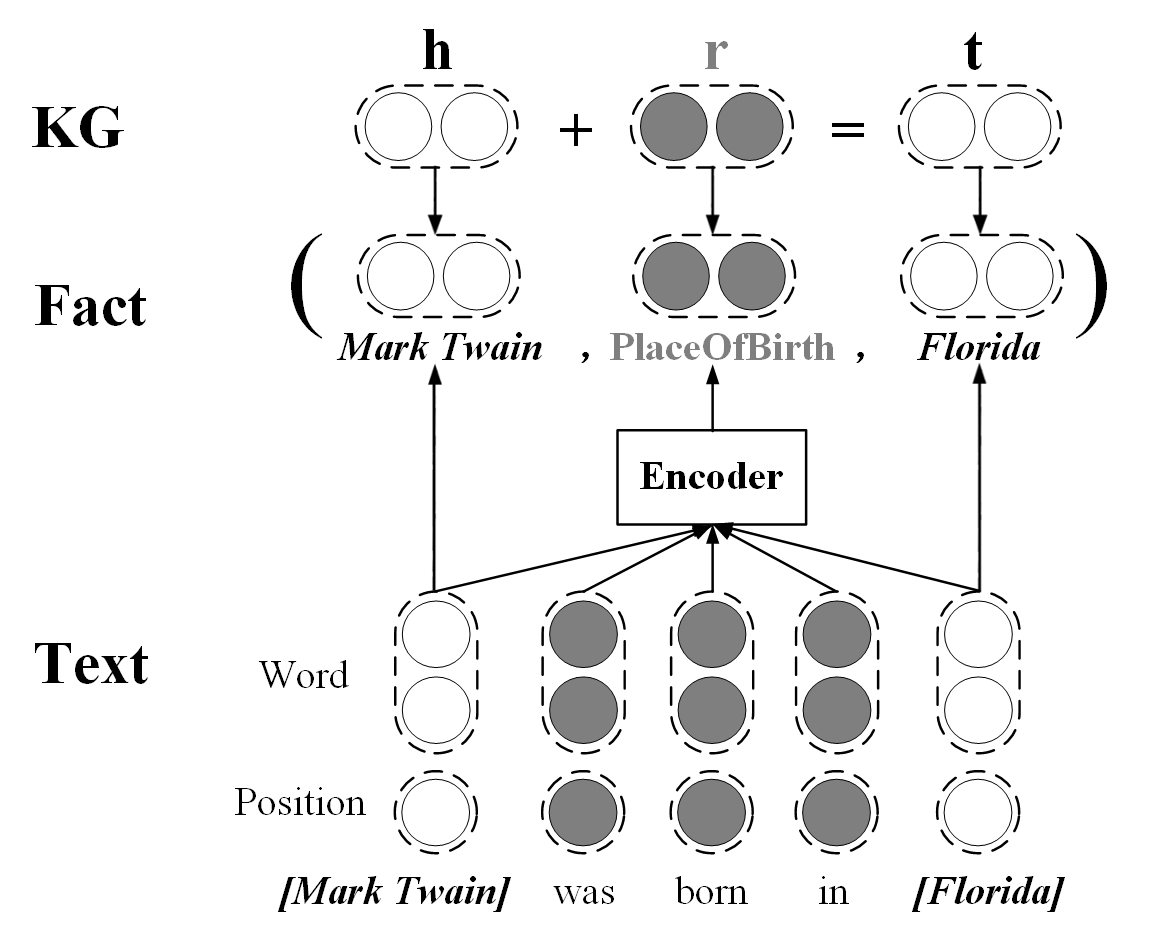
\includegraphics[width=0.9\columnwidth]{figures/ch3/joint.jpg}
\caption{基于并行的知识图谱与文本模型联合学习框架}
\label{fig:joinglearning}
\end{figure}

\section{算法框架}
在这一章节的内容里,论文主要介绍我们提出的基于并行的知识图谱与文本模型联合学习框架。内容包括以下几点:(1)联合框架下知识图谱与文本表示的统一形式;(2)知识图谱表示学习模型;(2)文本关系表示学习模型;(3)基于知识的跨句注意力机制;(4)初始化及实现细节,整体的框架结构也可以在图\ref{fig:joinglearning}中看到。从框架结构图中可以发现,在整个框架中,我们进行了大量的嵌入表示融合工作。这些融合工作包含了知识图谱与文本表示在模型形式上的统一,词与实体、关系与文本关系在嵌入向量上的统一等等。得益于这些统一的归纳与抽象,我们可以通过使用统一空间学习嵌入表示的方式来进行联合学习。联合学习支持模型间的参数共享,从而使得原本分离的模型在合并后可以相互影响并一定程度的促进各自效果提升。在介绍具体细节之前,我们仍然先引入一些符号体系和重要概念。

\subsection{符号体系和重要概念}

与大规模知识图谱表示学习框架一样,我们在这里同样将整个知识图谱定义为一个由实体集、关系集和事实三元组集合共同组成的大集合,即$G = \{E, R, T\}$,这里$E$、$R$和$T$分别表示实体集合、关系集合和事实三元组集合。对于事实三元组集合中的任意事实$(h, r, t) \in T$,这个三元组表明头实体$h \in E$和尾实体$t \in E$之间存在一个逻辑上的关联$r \in R$。

和知识图谱$G$相对应的是文本,这里我们将文本数据定义为$D$。$D$是文本数据的集合,集合中的元素是大量的文本句子,这些句子构成的词汇表被定义为$V$。对于文本数据集合$D$中的任意一个句子$s$,$s$被定义为一个由若干词汇表$V$中单词构成的词语序列$s = \{w_1, \ldots, w_n\}, w_i \in V$,$n$为句子的长度也是词语序列中单词的数量。在每个句子中有两个标注出的实体,且这个句子本身的文本内容可以叙述实体间的潜在语义关联$r_s \in R$。对于文本实体和语义关系的具体标注方法将会在章节\ref{sec:alignment}处被介绍。

由于表示学习会将实体和关系都嵌入到连续空间中去并用对应的向量来表示他们的语义信息,所以对于任意的实体或者关系$h, t \in E$或$r \in R$,我们都用它们的加粗字母$\mathbf{h}, \mathbf{t}, \mathbf{r} \in \mathbb{R}^{k_w}$来表示它们的向量,这里的向量也可以称为嵌入、嵌入向量、表示、嵌入表示等。对于任意单词$w \in V$,我们同样用加粗字母$\mathbf{w}\in \mathbb{R}^{k_w}$来表示其向量。$k_w$是这些单词、实体与关系的嵌入表示维度。

\subsection{联合学习的整体模式}
\label{sec:joint}

对于整个联合学习框架,我们希望框架可以支持下面的模型能够在一个统一的连续空间内同时学到实体、关系以及单词的嵌入表示,并通过这样的联合约束使得特征可以在知识图谱和文本间进行共享和传递。我们将所有的嵌入表示以及模型中涉及的变量都定义为模型参数,并用符号$\theta = \{\theta_E, \theta_R, \theta_V\}$来表示,其中$\theta_E, \theta_R, \theta_V$分别是实体、关系、单词的嵌入向量。如果将我们对框架的性能要求形式化的话,模型需要做的就是找到一组最优的参数$\hat{\theta}$满足
\begin{equation}
\hat{\theta} = \mathop{\arg\max}_{\theta} P(G, D | {\theta})
\end{equation}
这里$\theta_E, \theta_R, \theta_V$是之前定义的嵌入。$P(G, D | {\theta})$ 是一个定义出的条件概率,用来刻画在给定实体、关系与单词的嵌入$\theta$的情况下,嵌入对图谱与文本的拟合能力。直观点讲,模型的任务就是找到最好的嵌入表示能够最大程度的拟合给定的知识图谱结构以及文本语义信息。而条件概率$P(G, D | {\theta})$又可以进一步被分解为
\begin{align}
\label{eq:topeq}
P(G,D|{\theta}) = P(G|{\theta_E,\theta_R})P(D|{\theta_V})
\end{align}

$P(G|\theta_E, \theta_R)$ 被用来从知识图谱$G$中学习结构特征,并得到实体和关系的嵌入表示。这个式子的物理意义就是希望模型能够最大限度的让知识图谱$G$中的事实概率变大,关于此部分的详细内容将会在章节\ref{sec:kg}中展开。

$P(D|{\theta_V})$ 被用来从文本信息$D$中学习文本特征,并得到单词与语义关系的嵌入表示。这个式子的物理意义就是希望模型能够最大限度的让$D$中句子的语义信息与其描述的语义关系相对应,关于此部分的详细内容将会在章节\ref{sec:relation}中展开。

我们将知识图谱的概率定义为其包含的事实的概率,将文本的概率定义为语义信息与语义关系对应的概率,并对原概率式进行变换,得到
\begin{align}
 &P(G|{\theta_E,\theta_R})  = \prod_{(h,r,t) \in G}P((h, r, t)|{\theta_E, \theta_R}), \\
 &P(D|{\theta_V})  = \prod_{s \in D}P((s, r_s)|{\theta_V})
\end{align}
这里$P((h, r, t)|{\theta_E,\theta_R})$定义了知识图谱$G$中事实三元组在已知实体关系嵌入下的条件概率,而$P((s, r_s)|{\theta_V})$则定义了在已知单词嵌入的情况下,$D$中句子$s$能准确描述语义关系$r_s$的条件概率。

\subsection{知识图谱表示学习模型}
\label{sec:kg}

对于知识图谱表示学习,我们在之前的工作中也进行了详细的叙述,其主要任务就是通过将实体和关系表示为空间中的嵌入向量从而能够抓取语义关联。在章节\label{sec:joint}里我们已经将这个任务落实到对事实三元组条件概率进行优化的目标上。和Lin\cite{Lin2016Knowledge}一致,我们将优化条件概率$P((h, r, t)|{\theta_E, \theta_R})$转化为优化$P(h|(r, t),{\theta_E, \theta_R})$、$P(t|(h, r),{\theta_E, \theta_R})$以及$P(r|(h, t),{\theta_E, \theta_R})$。

对于每一个知识图谱$G$中的实体对$(h, t)$,我们定义出一个潜在关系向量$\mathbf{r}_{ht}$来表达实体向量$\mathbf{h}$到实体向量$\mathbf{t}$之间的变换,具体形式如下:
\begin{equation}
\textbf{r}_{ht} = \textbf{t} - \textbf{h}
\end{equation}
与此同时,对于知识图谱$G$中的任意三元组$(h, r, t) \in T$,对应存在一个显式的关系$r$来描述$h$与$t$的关系。所以我们可以将三元组的能量函数定义为
\begin{align}
\label{eq:kg_distance}
f_r(h, t) & = b - \lVert \textbf{r}_{ht} - \textbf{r} \rVert  
\\\nonumber
		& = b - \lVert (\textbf{t} - \textbf{h}) - \textbf{r}  \rVert
\end{align}
这里,$b$是一个常数偏移量,通常在$7$左右。这个式子表明,我们期望三元组集合$T$中的任意三元组$(h, r, t)$都有$\textbf{h} + \textbf{r} \approx \textbf{t}$。

基于这个能量函数,我们以$P(h|(r, t),{\theta_E, \theta_R})$为例来形式化的给出$T$中三元组的条件概率:
\begin{align}
P(h|(r, t),{\theta_E, \theta_R}) = \frac{\exp(f_r(h, t))}{\sum_{h' \in E} \exp(f_r(h', t))}
\end{align}
以此类推,我们按照同样的形式可以定义$P(t|(h, r), {\theta_E, \theta_R})$和$P(r|(h, t),{\theta_E, \theta_R})$。实际上,无论是理念还是实际模型,这个条件概率的表达任务和 TransE 是一致的,只是不再是基于边界值优化而是基于条件概率优化。所以,我们将这个模型命名为 Prob-TransE。

为了体现我们联合学习的模式可以适应多种知识图谱的表示学习模型,我们也引入了 TransD 来对知识图谱中三元组进行编码和嵌入,具体形式如下:
\begin{align}
&\textbf{r}_{ht} = \textbf{t}_{r} - \textbf{h}_{r}, \\\nonumber
&\textbf{h}_{r}  = \textbf{M}_{rh}\textbf{h},\\\nonumber 
&\textbf{t}_{r} = \textbf{M}_{rt}\textbf{t}, \\\nonumber
&\textbf{M}_{rh} = \textbf{r}_p\textbf{h}_p^{\top}+\textbf{I}^{k_r \times k_w},	\\\nonumber
&\textbf{M}_{th} = \textbf{r}_p\textbf{t}_p^{\top}+\textbf{I}^{k_r \times k_w}
\end{align}
这里$\textbf{r}_p \in \mathbb{R}^{k_r} $和$\textbf{h}_p, \textbf{t}_p \in \mathbb{R}^{k_w}$都是用来进行映射的工作向量。出于实验上的简化,关系嵌入维度$k_r$和实体嵌入维度$k_w$在我们的框架下被默认为是一样的值,在实际操作中往往也是采用了这样的设定。类似于 Prob-TransE,我们将基于 TransD 进行条件概率优化的知识图谱表示学习模型命名为 Prob-TransD。


\begin{figure}[t]
\centering
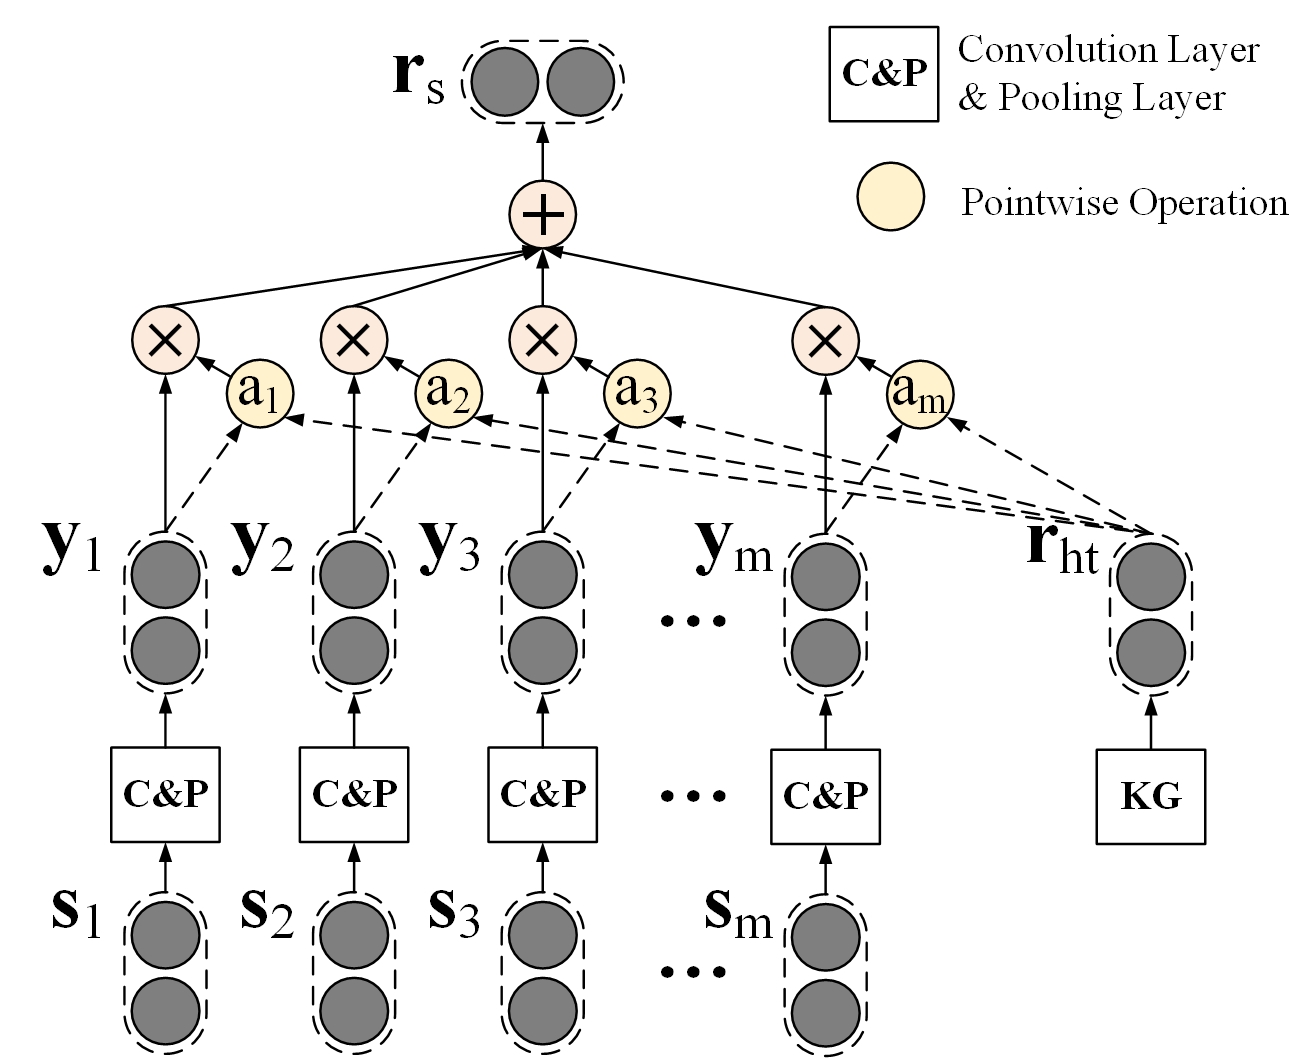
\includegraphics[width=0.9\columnwidth]{figures/ch3/cnn.jpg}
\caption{基于知识注意力机制的卷积神经网络模型}
\label{fig:cnn}
\end{figure}


\begin{figure}[h]
\centering
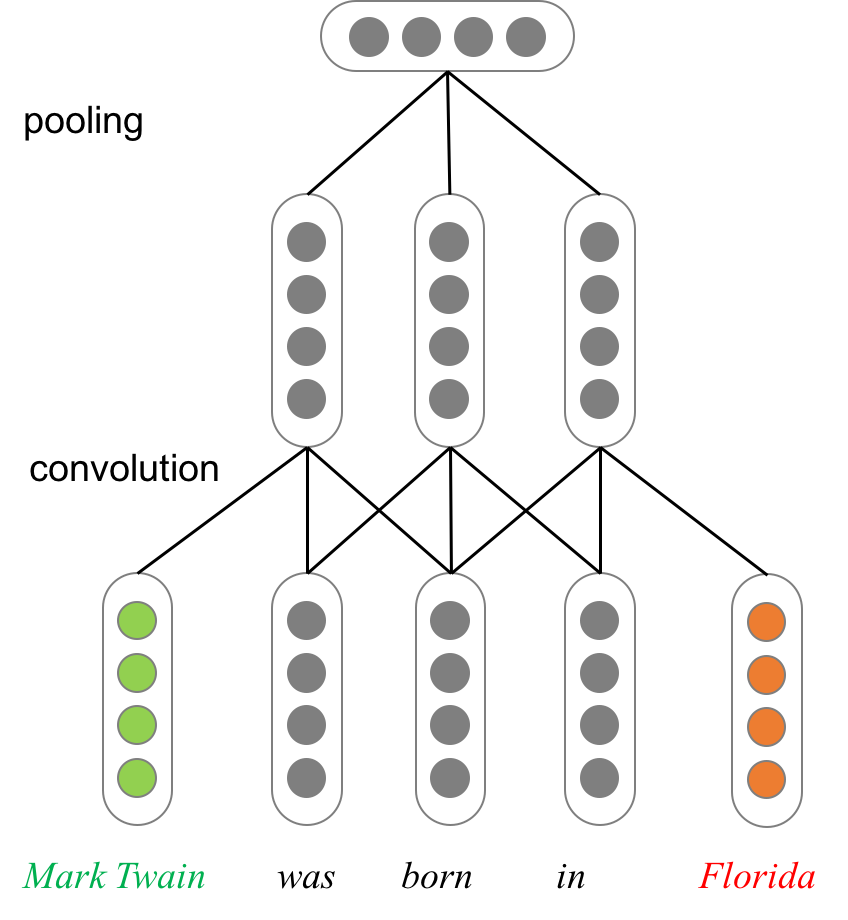
\includegraphics[width=0.7\columnwidth]{figures/ch3/cnn_concrete.png}
\caption{卷积层和池化层的结构示意图}
\label{fig:conv_pooling}
\end{figure}





\subsection{文本关系表示学习模型}
\label{sec:relation}

给定一个包含两个实体的句子,句子中的词以及句子本身的语义信息很大程度上可以揭开实体间的关系,比如``马克吐温出生于佛罗里达州''直接表明了\emph{马克吐温}和\emph{佛罗里达州}是人与籍贯的关系。Zeng、Toutanova以及Lin\cite{zeng2014relation,toutanova2015representing,lin2016neural},他们在各自的工作中都开始尝试使用神经网络来挖掘这样的语义信息,并且将语义信息描述的关系嵌入到低维空间中用来进行关系抽取。和他们的工作\cite{zeng2014relation,toutanova2015representing,lin2016neural}相似,我们也采用了卷积神经网络 CNN 对文本关系进行表示学习。

图\ref{fig:cnn}描述了我们卷积神经网络的整个结构,也是文本关系表示学习模型的整个结构。对于任意一个标注了实体对$(h, t)$的句子$s$,如果实体对之间的关系为$r_s$的话,神经网络结构会以句子$s$的词语序列向量$\mathbf{s} = \{\mathbf{x}_1, \ldots, \mathbf{x}_n \}$作为输入。输入的句子向量在通过卷积神经网络中卷积与池化两层操作后,输出一个文本意义描述的关系向量$\mathbf{y}$。由于存在多个句子标注了相同的实体,我们设置了一个基于知识图谱的注意力机制,用来在这些句子输出的基础上进行加权合并,然后得到一个全局的文本关系表示$\mathbf{r}_s$。对于句子的语义信息能在多大程度上描述文本关系,在经过一层多项逻辑斯特回归之后,我们用以下的能量函数来刻画:
\begin{equation}
\mathbf{o} = \mathbf{M}\mathbf{r}_s,
\label{eq:cnn_distance}
\end{equation}
这里$\mathbf{M} \in \mathbb{R}^{\|R\| \times k_c} $是一个关系表示矩阵用来求得$\mathbf{r}_s$在不同的关系上的能量评分,$k_c$是隐层向量的维度,最后我们可以定义一个条件概率$P((s, r_s)|{\theta_V})$:
\begin{equation}
P((s, r_s)|{\theta_V}) = \frac{\exp(\mathbf{o}_{r_s})}{\sum_{r \in R} \exp(\mathbf{o}_{r})}
\label{eq:cnn_distance1}
\end{equation}

我们的文本关系表示模型就是由这几个部分构成的,包括输入层、卷积层、池化层、基于知识的注意力机制以及刚才介绍的分类层,相关细节将在下面一一展开。


\subsubsection{输入层}
 


We simply concatenate textual word embeddings and word position embeddings to build the input for CNN:
\begin{equation}
\mathbf{s} = \{[\mathbf{w}_1;\mathbf{p}_1],\ldots, [\mathbf{w}_n;\mathbf{p}_n]\}.
\end{equation}



给定一个含有$n$个单词的句子$s$,$s = \{ w_1, \ldots , w_n\}$,输入层的功能就是将$s$中的所有单词转化成对应的输入词向量$\mathbf{s} = \{ \mathbf{x}_1, \ldots , \mathbf{x}_n \}$。对于给定句子$s$中的任意一个单词$x_i$,其输入向量$\mathbf{x}_i$由两个实向量构成,一个是它的文本词向量$\mathbf{w}_i$,另一个是它的位置向量$\mathbf{p}_{i}$。

文本词向量可以将词的语义信息编码到低维空间中,并且通常会通过大量文本预先训练获得。大量的实验表明,以预先训练好的词向量作为网络输入可以有效提升神经网络的模型效果。在我们的工作中,词向量通过 Skip-Gram \cite{mikolov2013efficient}在大规模文本语料上提前训练获得。

位置向量的概念首次被提出是在 Zeng \cite{zeng2014relation} 的工作中。位置向量是一个可以表明给定单词与句子标注实体之间相隔距离的特征。举个例子,``\emph{马克吐温}出生于\emph{佛罗里达州}''中,\emph{马克吐温}与\emph{佛罗里达州}是标注出的实体,\emph{出}离\emph{马克吐温}和\emph{佛罗里达州}的距离分别为$1$和$-3$。我们会将这些距离映射到维度$k_p$的连续空间上。对于句子$s$中给定的单词$w_i$,它的位置向量为$\mathbf{p}_i = [\mathbf{p}^h_i, \mathbf{p}^t_i]$, $\mathbf{p}^h_i, \mathbf{p}^t_i \in \mathbb{R}^{k_p}$,其中$\mathbf{p}^h_i$ 和 $\mathbf{p}^t_i$分别是到头实体以及尾实体之间的距离向量。

接着我们合并词向量$\mathbf{w}_i \in \mathbb{R}^{k_w} $与位置向量$\mathbf{p}_i \in \mathbb{R}^{k_p \times 2} $得到最终的输入向量$\mathbf{x}_i \in \mathbb{R}^{k_i} (k_i = k_w + k_p \times 2)$,从而卷积神经网络的输入为:
\begin{align}
\mathbf{s} & = \{\mathbf{x}_1,\ldots, \mathbf{x}_n\} \\\nonumber
&=\{[\mathbf{w}_1;\mathbf{p}_1],\ldots, [\mathbf{w}_n;\mathbf{p}_n]\}.
\end{align}

\subsection{卷积层}

卷积层将输入层的输出$\mathbf{s}$作为该层的输入,通过卷积层内的操作后导出为隐层向量$\mathbf{h}$。在卷积层中,我们在输入的序列向量$\mathbf{s}$上滑动一个尺寸为$m$的窗口。在每次窗口滑动中,我们可以采样得到一个局部的组合向量$\mathbf{\hat{x}}_i$:
\begin{equation}
\mathbf{\hat{x}}_i = \big[ \mathbf{x}_{i - \frac{m-1}{2}}; \ldots ; \mathbf{x}_i; \ldots ;\mathbf{x}_{i + \frac{m-1}{2}} \big],
\end{equation}
这个组合向量就是通过将输入序列向量$\mathbf{s}$在窗口中以$\mathbf{x}_i$为中心的$m$个向量组合而成。然后,我们将这个组合向量$\mathbf{\hat{x}}_i$进行线性变换以及激活从而得到隐层函数$\mathbf{h}_i$
\begin{equation}
\mathbf{h}_i = \tanh(\mathbf{W}\mathbf{\hat{x}}_i + \mathbf{b}),
\end{equation}
这里,$\mathbf{W} \in \mathbb{R}^{k_c \times mk_i}$是卷积层的卷积核矩阵,$\mathbf{b} \in \mathbb{R}^{k_c}$是卷积层的偏移向量,$k_c$是隐层向量$\mathbf{h}_i$的维度。

\subsection{池化层}

在池化层中,一个最大池化操作在隐层向量${\mathbf{h}_1, \ldots , \mathbf{h}_n}$上被实施来获得最后的输出向量$\mathbf{y} \in \mathbb{R}^{k_c} $,具体的过程如下:
\begin{equation}
\mathbf{y}_{j} = \max \{\mathbf{h}_{1,j}, \ldots, \mathbf{h}_{n,j} \},
\end{equation}
这里,$\mathbf{y}_{j}$是输出向量$\mathbf{y}$的第$j$维的值,$\mathbf{h}_{i,j}$是第$i$个隐向量$\mathbf{h}_i$的第$j$维的值。池化层的主要作用在于对全局的特征进行汇总。在卷积层中,卷积实际上是对局部的语义的特征提取,但一个句子的语义实际上不是局部的而是一个全局的,池化的作用正是在每个局部采样中的每个维度上选取一个信号最为强烈的采样,从而最后能够汇总得到全局的语义特征,这是至关重要的一个步骤。

\subsection{基于知识的跨句注意力机制}

对于知识图谱中任意一个三元组$(h, r, t) \in T$,实际上可能存在若干个句子会包含这个三元组中的实体对$(h, t)$,并且这些句子的语义预示着实体对具有关系$r$。经过输入层、卷积层、池化层,这些句子已经有了输出向量${\mathbf{y}_1, \ldots , \mathbf{y}_m}$,$m$为包含这些实体对的句子数量。对于这些句子,我们认为其中的某些句子对最后的文本关系表示学习会更具有贡献性,所以我们需要一个机制来选取这些重要的句子且规避噪音。

在这里我们通过引入知识图谱中的潜在关系向量$\mathbf{r}_{ht} \in \mathbb{R}^{k_w} $来神经网络进行一个基于知识的注意力机制,从而强化重要句子的影响,具体形式如下:
\begin{align}
\mathbf{e}_j & = \tanh(\mathbf{W}_s\mathbf{y}_j+\mathbf{b}_s), \\\nonumber
a_j & =\frac{\exp(\mathbf{r}_{ht}\cdot\mathbf{e}_j)}{\sum_{k = 1}^{m} \exp(\mathbf{r}_{ht}\cdot\mathbf{e}_k)}, \\\nonumber
\mathbf{r}_s & = \sum_{j = 1}^{m} a_j\mathbf{y}_j,
\end{align}
这里,$\mathbf{W}_s \in \mathbb{R}^{k_w \times k_c}$是一个权重矩阵用来将前几层的输出向量转换到图谱空间中,$\mathbf{b}_s \in \mathbb{R}^{k_w}$则是线性变换的偏移向量。$a_j$是第$j$个句子输出向量$\mathbf{y}_j$在整个注意力机制结算后得到的权重评价。我们通过每个句子输出向量的权重来对这些向量进行加权求和从而得到一个全局的文本关系嵌入表示$\mathbf{r}_s$。有了全局的嵌入向量后,我们可以将向量$\mathbf{r}_s$带入式\ref{eq:cnn_distance}以及式\ref{eq:cnn_distance1}中进行分类。



\subsection{初始化及实现细节}
\label{sec:detail}
在这一部分,我们主要介绍我们的模型在具体训练以及优化过程中的一些细节操作。对于我们以条件概率式\ref{eq:topeq}为形式的任务目标,我们定义了一个对数似然函数来作为我们的优化目标,
\begin{align}
\mathcal{L}_{\theta}(G, D) & = \log P(G,D|{\theta}) + \lambda \lVert \theta \rVert_2 \\\nonumber
 & = \log P(G|{\theta_E, \theta_R}) + \log P(D|{\theta_V}) \\\nonumber
 & + \lambda \lVert \theta \rVert_2
\end{align}
这里,$\lambda$是一个超参,$\lVert \theta \rVert_2$是一个$L_2$距离的约束条件。我们的所有模型,包括 Prob-TransE 和 Prob-TransD 以及 CNN 都是通过随机梯度下降(stochastic gradient descent,SGD)算法来进行优化。值得注意的是,我们的损失函数的梯度会被传递到输入层的词向量上,因为这样才能将知识图谱的特征嵌入到词向量中。我们实现了一个多线程同步训练的模式来进行图谱和文本两方面的模型同时训练。每个线程控制一个模型以及所使用的训练数据。多个模型在内存上共用词、实体以及关系的嵌入表示,且不加锁,梯度直接反馈到向量上。







